\documentclass[aspectratio=169]{beamer}
\geometry{paperwidth=160mm,paperheight=100mm}
\usepackage{beamerthemesidebar}
\usepackage{hyperref}
\usepackage{color}
\usepackage{multimedia}
\usepackage{colortbl}
\usepackage{amsmath}
\usepackage{empheq}
\usepackage{cancel}
\usepackage{amssymb}
\usepackage{amsfonts}
\usepackage{lipsum}
\usepackage{tcolorbox}
\usepackage{tabularx}
\usepackage{caption}
\usepackage{bm}

\setbeamersize{sidebar width right=0pt}
\setbeamertemplate{footline}[frame number]
%
\definecolor{orange}{RGB}{250,167,12}
\definecolor{yellow}{RGB}{246,250,12}
\definecolor{green}{RGB}{128,238,1}
\definecolor{black}{RGB}{0,0,0}
\definecolor{blue}{RGB}{0,0,255}
\definecolor{red}{RGB}{255,0,0}
\definecolor{sepia}{RGB}{94,38,18}
\newcommand{\ve}[1]{{\rm\bf {#1}}}
\newcommand{\q}[1]{\textcolor{blue}{#1}}
\newcommand{\blue}[1]{\textcolor{blue}{#1}}
\newcommand{\sepia}[1]{\textcolor{sepia}{#1}}
\newcommand{\red}[1]{\textcolor{red}{#1}}
\newcommand{\green}[1]{\textcolor{green}{#1}}
\newcommand{\yellow}[1]{\textcolor{yellow}{#1}}
\newcommand{\orange}[1]{\textcolor{orange}{#1}}
\definecolor{burlywood}{RGB}{255,211,155}
\definecolor{chocolate}{RGB}{255,127,36}
\definecolor{tan}{RGB}{210,180,140}
%
\def\onethird{{\textstyle{1\over3}}}
\def\twothirds{{\textstyle{2\over3}}}
\def\fourthirds{{\textstyle{4\over3}}}
\def\onehalf{{\textstyle{1\over2}}}
\def\threehalfs{{\textstyle{3\over2}}}
%
\newcommand{\pd}{\partial}
\newcommand{\aMLT}{\alpha_{\rm MLT}}
\newcommand{\Fconv}{F_{\rm conv}}
\newcommand{\Frad}{F_{\rm rad}}
\newcommand{\Ftot}{F_{\rm tot}}
\newcommand{\Hp}{H_p}
\newcommand{\prad}{p_{\rm rad}}
\newcommand{\pgas}{p_{\rm gas}}
%
\title{Theoretical Astrophysics I: Physics of Sun and Stars\\
Lecture 6: Radiative Energy Transport}
\author{\texorpdfstring{\sepia{Petri K\"{a}pyl\"{a} Ivan Mili\'{c}}\newline\blue{\url{pkapyla, milic@leibniz-kis.de}}}{}}
\institute{Institut f\"ur Sonnenphysik - KIS, Freiburg}
\date{\today}
%
\begin{document}
\frame{\titlepage}

% Few general remarks on photons vs particles 
% Description of radiation field: angle and wavelength dependence
% RTE Kirchoffs Law, Planck Law
% optical depth, source function etc. 
% Few simple solutions 
% Diffusion approximation
% Opacity sources 
% Misc 


\section{General remarks}
%
\frame{
\frametitle{Brief recap}
\begin{minipage}{0.55\linewidth}
\begin{itemize}
\item We started with describing observed properties of the stars. One quantity that we measure (and want to reproduce) is the \textbf{luminosity}, and conversely \textbf{flux} (or specific flux).
\item We wrote down equations that govern stellar structure and evolution. Solving them for proper boundary conditions will yield the structure of a star: $p(r)$, $T(r)$, $\rho(r)$, $F(r)$, etc...
\item Analyzing their variation in time allows us to model stellar evolution.
\item We spent last two lectures talking about a difficult problem of convection. But there is another way to transport energy: via \textbf{radiation}.
\end{itemize}
\end{minipage}
\begin{minipage}{0.44\linewidth}
\begin{figure}
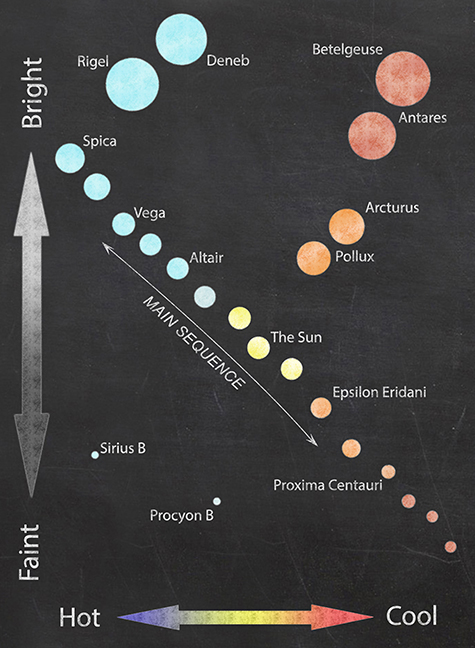
\includegraphics[width=6cm]{figures/hr_simple.jpg}
\caption*{HR diagram}
\end{figure}
\end{minipage}
}
%
\frame{
\frametitle{Photons vs particles}
\begin{minipage}{0.5\linewidth}
\begin{itemize}
\item It is obvious that radiation can carry energy. 
\item We treat radiation using photons, but they are clearly different from atoms, molecules, ions and electrons. 
\item Photons do not have mass and move with speed of light. 
\item The number of photons is not conserved. 
\item Photons can also be treated like a gas (e.g. see the derivation of Stefan-Boltzmann law by Boltzmann)
\item They still observe conservation of energy, momentum, angular momentum, etc.
\end{itemize}
\end{minipage}
\begin{minipage}{0.49\linewidth}
\begin{figure}
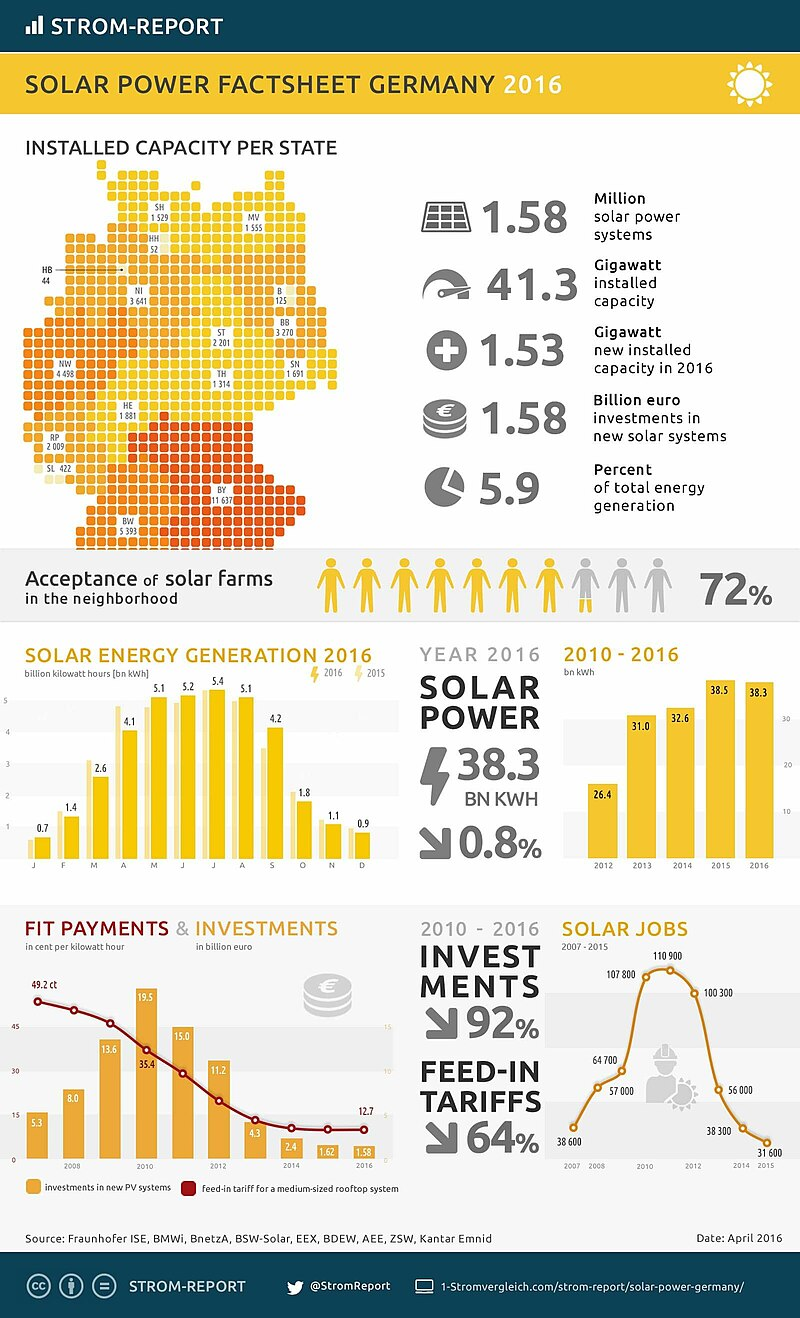
\includegraphics[width=4.5cm]{figures/solar_power.jpg}
\caption*{Credits: Strom Report}
\end{figure}
\end{minipage}
}
%
\frame{
\frametitle{Photons vs particles}
\begin{minipage}{0.5\linewidth}
\begin{itemize}
\item It will be essential to understand photon-matter interaction. As Ivan Hubeny said: 
\item \emph{...In other words radiation in fact determines the structure of the medium yet the medium is probed only by this radiation.}
\item Radiation: constituent in energy transport (and equation of state).
\item Also: diagnostics that allows us to understand physical properties of the medium.
\item Contrary to the lab: we need to treat wavelength and angular dependence of the radiation field.
\end{itemize}
\end{minipage}
\begin{minipage}{0.49\linewidth}
\begin{figure}
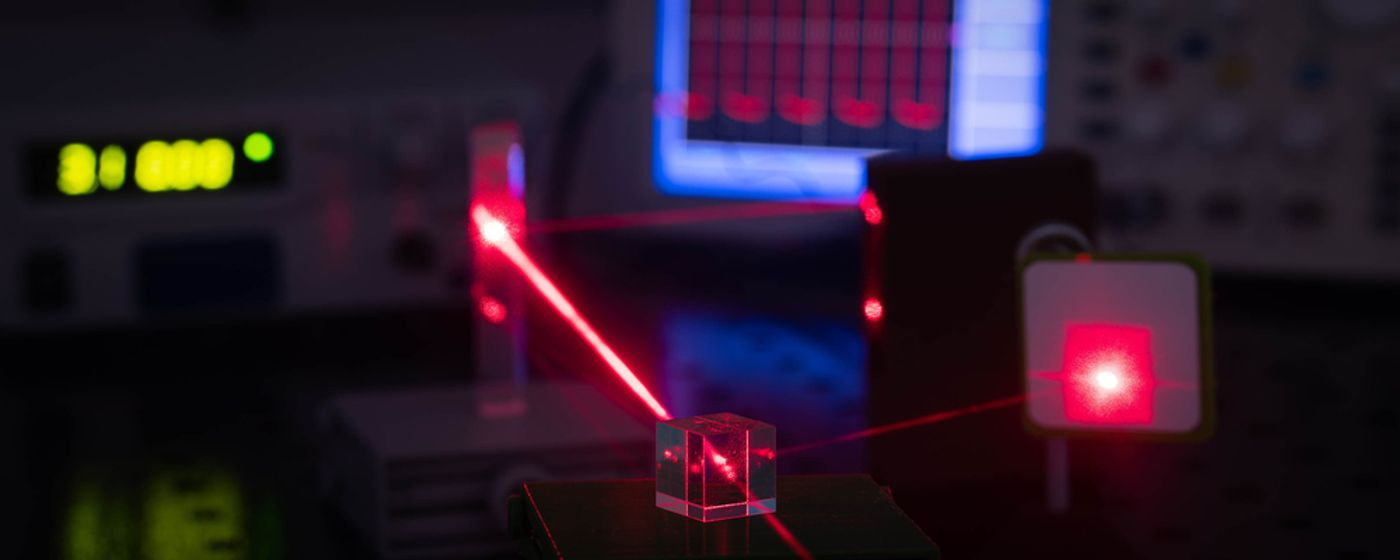
\includegraphics[width=4.5cm]{figures/laser_roots.jpg}\\
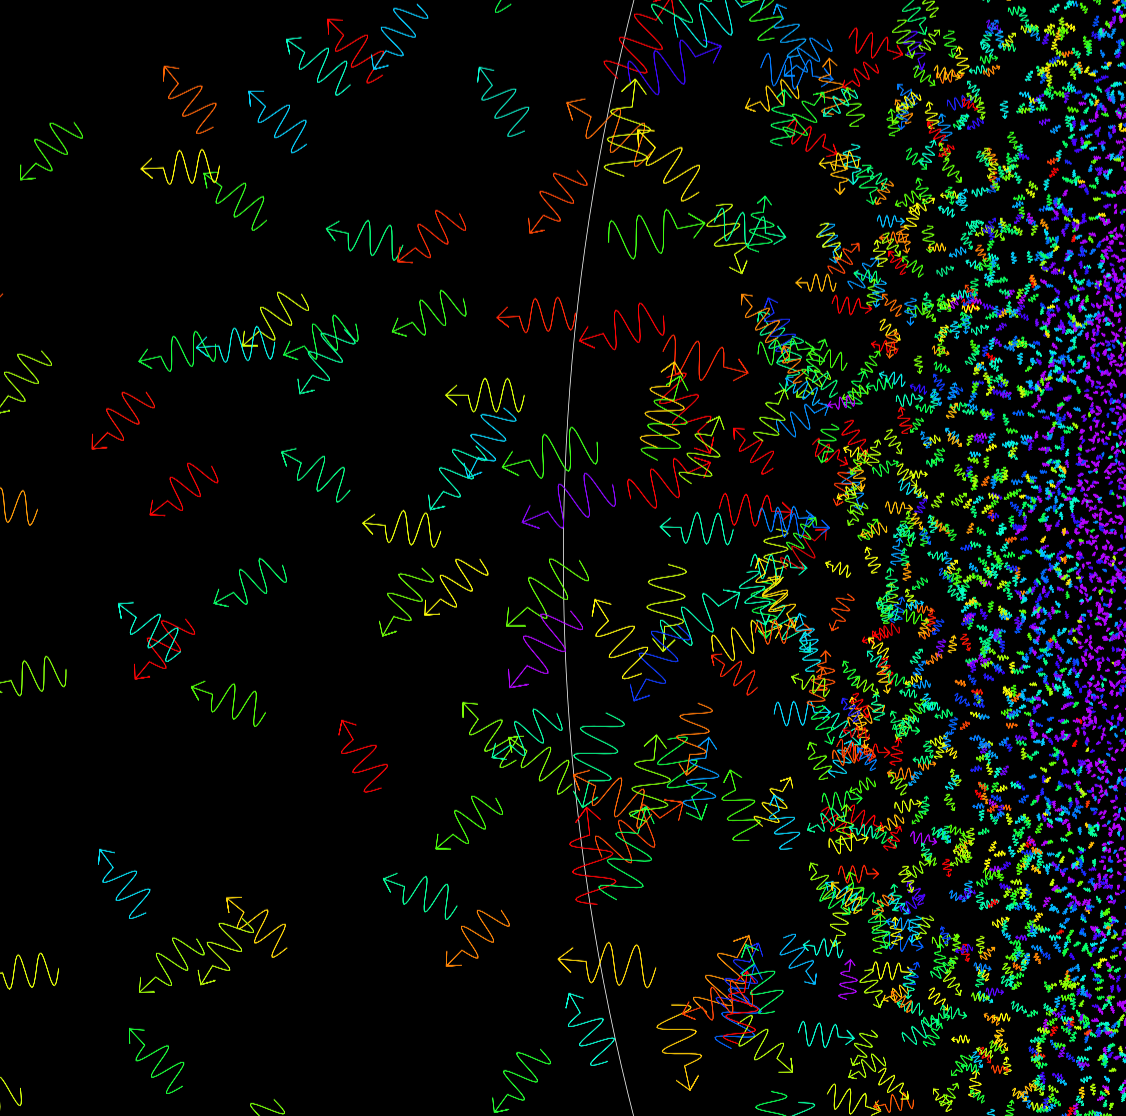
\includegraphics[width=4.5cm]{figures/sa.png}
\caption*{Credits: LabRoots.com (up), Prof. Rob Rutten (bottom)}
\end{figure}
\end{minipage}
}
%
\section{Radiation field}
%
\frame{
\frametitle{Specific monochromatic intensity}
\begin{minipage}{0.5\linewidth}
\begin{itemize}
\item We need to treat wavelength and angular dependence of the radiation field
\item Intensity: energy transported through given area in given time per given solid angle and frequency/wavelength bin (note the deprojection factor $\cos \theta$).
\begin{equation}
I_\nu = \frac{dE}{dS\,dt\,d\Omega\,d\nu\,\cos \theta}
\end{equation}
\item Going to number of photons:
\begin{equation}
n(\theta,\phi\,\nu) = \frac{I_\nu}{h\nu}
\end{equation}
\end{itemize}
\end{minipage}
\begin{minipage}{0.49\linewidth}
\begin{figure}
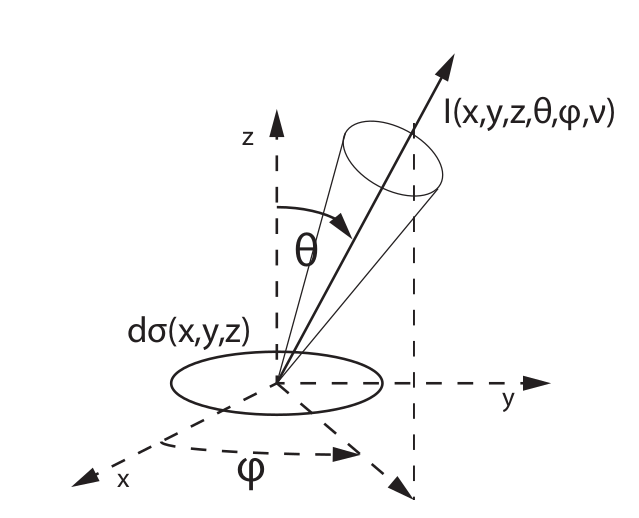
\includegraphics[width=6.0cm]{figures/spec_int.png}
\caption*{Credits: IM thesis (2014, University of Belgrade)}
\end{figure}
\end{minipage}
}
%
\frame{
\frametitle{Other ``moments'' of the radiation field}
\begin{minipage}{0.5\linewidth}
\begin{itemize}
\item Intensity fully describes the radiation field (without polarization). But often we need some derived quantities:
\item Mean intensity:
\begin{equation}
J_\nu = \frac{1}{4\pi}\oint I_\nu (\theta,\phi) \sin \theta d \theta d \phi
\end{equation}
\item Flux (in $z$ direction):
\begin{equation}
\mathcal{F}_\nu = \oint I_\nu (\theta,\phi) \cos \theta \sin \theta  d \theta d \phi
\end{equation}
\end{itemize}
\end{minipage}
\begin{minipage}{0.49\linewidth}
\begin{figure}
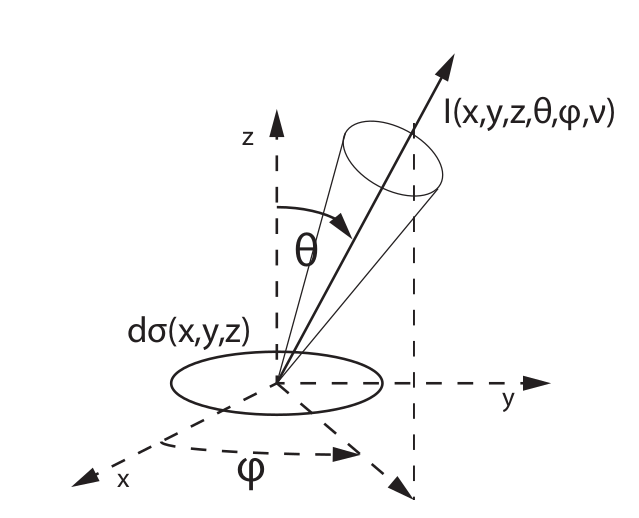
\includegraphics[width=6.0cm]{figures/spec_int.png}
\caption*{Credits: IM thesis (2014, University of Belgrade)}
\end{figure}
\end{minipage}
}
%
\frame{
\frametitle{Some de-confusion of the term flux}
\begin{itemize}
\item Typically we say that (spectral, monochromatic) flux is:
\begin{equation}
F_\nu = \frac{dE}{dt dS d\nu}
\end{equation}
\item But in the book typically:
\begin{equation}
F_\nu = \frac{dE}{dt d\nu} \rightarrow F = \frac{dE}{dt}
\end{equation}
But then, to make situation works, in stellar atmospheres theory flux is:
\begin{equation}
\mathcal{F}_\nu = \frac{dE}{dt dS d\nu}
\end{equation}
then astrophysical flux: 
\begin{equation}
F_\nu = \frac{1}{\pi}\frac{dE}{dt dS d\nu}
\end{equation}
and Eddington flux (which the book uses and calls the radiation flux) is:
\begin{equation}
H_\nu = \frac{1}{4\pi}\frac{dE}{dt dS d\nu} = \frac{1}{4\pi} \mathcal{F}_\nu
\end{equation}
\end{itemize}
}
%
\frame{
\frametitle{More moments of the radiation field}
\begin{itemize}
\item Mean intensity:
\begin{equation}
J_\nu = \frac{1}{4\pi}\oint I_\nu (\theta,\phi) \sin \theta d \theta d \phi
\end{equation}
\item Radiation flux:
\begin{equation}
\mathcal{H}_\nu = \frac{1}{4\pi} \oint I_\nu (\theta,\phi) \cos \theta \sin \theta  d \theta d \phi
\end{equation}
\item and the so called K-integral, which is proportional to the pressure of the radiation field:
\begin{equation}
\mathcal{K}_\nu = \frac{1}{4\pi} \oint I_\nu (\theta,\phi) \cos^2 \theta \sin \theta  d \theta d \phi = \frac{p_\nu c}{4 \pi}
\end{equation}
\item \textbf{Note that we can define all these in the frequency/wavelength-integrated form}

\end{itemize}
}
%
%
\frame{
\frametitle{More moments of the radiation field}
\begin{itemize}
\item Mean intensity:
\begin{equation}
J = \frac{1}{4\pi}\int_0^{\infty}\oint I_\nu (\theta,\phi) \sin \theta d \theta d \phi d\nu
\end{equation}
\item Radiation flux:
\begin{equation}
\mathcal{H} = \frac{1}{4\pi} \int_0^{\infty}\oint I_\nu (\theta,\phi) \cos \theta \sin \theta  d \theta d \phi d\nu
\end{equation}
\item and the so called K-integral, which is proportional to the pressure of the radiation field:
\begin{equation}
\mathcal{K} = \frac{1}{4\pi} \int_0^{\infty}\oint I_\nu (\theta,\phi) \cos^2 \theta \sin \theta  d \theta d \phi d\nu = \frac{p\,c}{4 \pi} 
\end{equation}
\item \textbf{Here we integrated over all frequencies}

\end{itemize}
}
%
\frame{
\frametitle{A quick question:}
\begin{itemize}
\item What would be the radiation flux if the intensity was isotropic?
\begin{equation}
\mathcal{H}_\nu = \frac{1}{4\pi} \oint I_\nu (\theta,\phi) \cos \theta \sin \theta  d \theta d \phi
\end{equation}

\end{itemize}
}
%
%
\frame{
\frametitle{A quick question:}
\begin{itemize}
\item What would be the radiation flux if the intensity was isotropic?
\begin{equation}
\mathcal{H}_\nu = \frac{1}{4\pi} \oint I_\nu (\theta,\phi) \cos \theta \sin \theta  d \theta d \phi
\end{equation}
\item A common substitute in this case is to integrate $\phi$ to $2\pi$ and then set $\cos \theta = \mu$ (this is again an another $\mu$).
\begin{equation}
\mathcal{H}_\nu = \frac{1}{2} \int_{-1}^{1} I_\nu (\mu) \mu d\mu = 0
\end{equation}
\item If the radiation is completely isotropic, there is no energy transport. In order to transport the energy outward toward the surface the radiation has to be slightly anisotropic.
\end{itemize}
}
%
\section{RTE}
%
\frame{
\frametitle{Modeling the radiation field}
\begin{minipage}{0.5\linewidth}
\begin{itemize}
\item Our task is not to model and understand intensity and its relationship with other physical quantities (density, temperature, pressure, chemical composition). For that we need to:
\item Understand the interaction between the radiation and matter (absorption, emission, scattering coefficients).
\item Mathematically express relationship between these coefficients and the intensity. 
\end{itemize}
\end{minipage}
\begin{minipage}{0.49\linewidth}
\begin{figure}
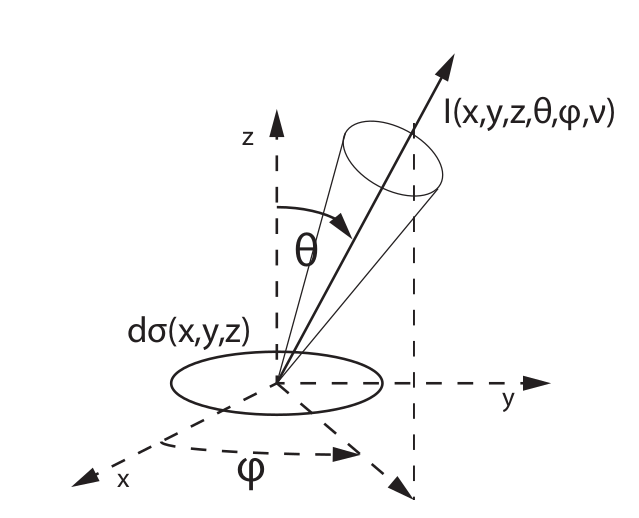
\includegraphics[width=6.0cm]{figures/spec_int.png}
\caption*{Credits: IM thesis (2014, University of Belgrade)}
\end{figure}
\end{minipage}
}
%
%
\frame{
\frametitle{Radiative Transfer Equation (RTE)}
\begin{minipage}{0.5\linewidth}
\begin{itemize}
\item This formulation is (more or less) due to Kirchhoff. The change of intensity ``along-the-ray'' over a distance $ds$ is:
\begin{equation}
dI_\nu = \eta_\nu ds - \chi_\nu I_\nu ds 
\end{equation} 
\item The terms of the right represent emission and \textbf{total} absorption (both true absorption and scattering) per unit volume.
\end{itemize}
\end{minipage}
\begin{minipage}{0.49\linewidth}
\begin{figure}
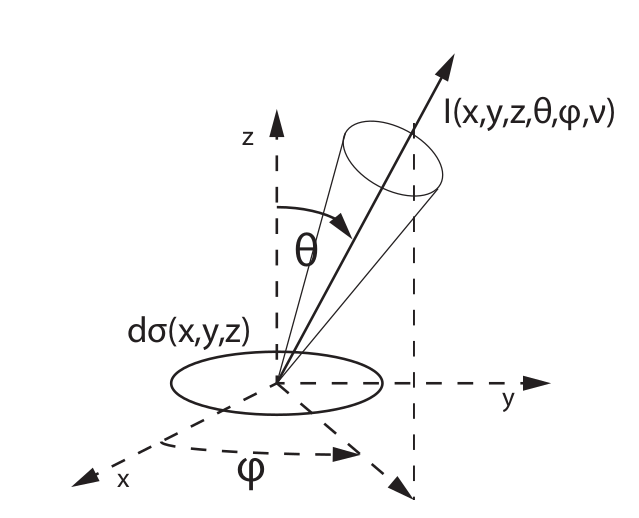
\includegraphics[width=6.0cm]{figures/spec_int.png}
\caption*{Credits: IM thesis (2014, University of Belgrade)}
\end{figure}
\end{minipage}
}
%

\end{document}



